\section{What}\label{sec:what}

\begin{wrapfigure}{R}{0.3\textwidth}
\centering
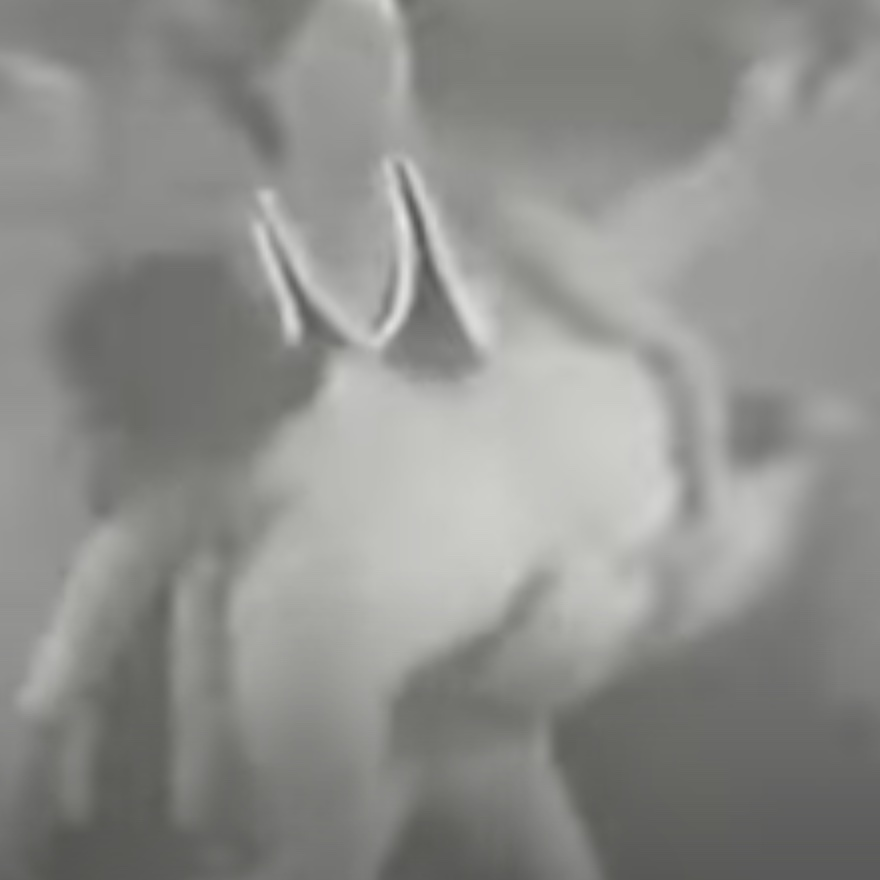
\includegraphics[width=0.25\textwidth]{images/what}
\end{wrapfigure}

So what is CI? A dance, a sport, acrobatics or martial arts?
Well, all of it, and none of it.

It could be considered a form of improvised partner dancing, a contemporary/postmodern dance form, an ``art-sport'', yet without any predefined choreography.
An exploration of one's body in relationship to others by using principles of sharing weight, touch, and movement awareness.
To play with the artistry of falling off balance and counterbalance, with gravity and physics.
To learn the mechanics of the body to handle someone's weight or to be lifted, along with breathing techniques.
At its core it involves mindfulness, sensing and collecting information which requires full present and attention.
And yes, it is even related to other improvisation practices like improvisation acting: the ``Yes, and \ldots'' concept expressed physically.

Emphasize is put on:
\begin{itemize}
	\item \textbf{Experimental dance}: practice-based research in dance laboratories
	\item \textbf{Theatrical form}: improvised performances and lectures-demonstrations
	\item \textbf{Educational tool}: training for professional dancers in improvisation
	\item \textbf{Awareness practice}: being able to listen to the subtleties in contact
	\item \textbf{Social dancing}: at informal gatherings called ``jams''
\end{itemize}

This art form is not only for the young and well-trained, as there is no real requirement for acrobatic performance.
The body just needs to be mobile and the bones bear some weight.

The founders decided to keep CI open to a broad community, thus it never has been institutionalised, neither is the name copyright protected.
Yet, [Contact Quarterly](https://contactquarterly.com) and [ECITE](http://www.ecite.org) can be considered the two main international forums ensuring the quality and continuity of CI.

There is a broad global community, which organizes social dances, so-called ``jams'', and practitioners often overlap with the ecstatic dance communities.

\subsection{Jams}\label{subsec:jams}

Jams, as stated already above, are social gatherings without any leader.
Occasions to meet other fellow practitioners, friends or strangers, old, young, experienced, novice.
They can be regularly in a studio for a few hours, or longer retreat jams for several days in spring resorts where it can be practiced at any hour of the day.

\subsection{Historically}\label{subsec:historically}

An early definition by Steve Paxton and others (CQ Vol. 5:1, Fall 1979):

A continuously evolving system of improvised movement.
Two bodies, communicating with each other in physical contact, creating a relationship with the physical laws (motion, gravity, momentum, inertia).
Sensitive, thus relaxed of unnecessary muscular tension, and willing to experience a natural flow.
Techniques may include: Rolling, falling, being upside down, following, supporting and giving weight.

A physical dialogue ranging from stillness to highly energetic exchange.
Alert enough to stay in an energetic state of physical disorientation, trusting your survival instincts.
A free play seeking for balanced movements, leading to a physical and emotional truth, shared in the moment, leaving you informed, centered, and enlivened

\subsection{Definitions}\label{subsec:definitions}

\textbf{Steve Paxton} himself stated in 1979: \textit{The exigencies of the form dictate a mode of movement which is relaxed, constantly aware and prepared, and onflowing. As a basic focus, the dancers remain in physical touch, mutually supportive and innovative, meditating upon the physical laws relating to their masses: gravity, momentum, inertia, and friction. They do not strive to achieve results, but rather, to meet the constantly changing physical reality with appropriate placement and energy.}

\textbf{Nancy Start Smith} once mentioned, it ``\textit{resembles other familiar duet forms, such as the embrace, wrestling, surfing, martial arts, and the Jitterbug (Lindy Hop and swing dances), encompassing a wide range of movement from stillness to highly athletic}''.

\textbf{Daniel Lepkoff} states about the core of CI, to ``\textit{put focus on bodily awareness and physical reflexes, rather than consciously controlled movements. Precedence of body experience first, and mindful cognition second, is an essential distinction between CI and other approaches to dance.}''


\textbf{Ray Chung} once announced in an workshop 2009 that CI is ``\textit{an open-ended exploration of the kinaesthetic possibilities of bodies moving through contact. Sometimes wild and athletic, sometimes quiet and meditative, it is a form open to all bodies and enquiring minds.}''

\subsection{Beyond CI}\label{subsec:beyond-ci}

CI is for sure not a pure \textbf{martial art}, as it has no claim to have any real fighting application.
Nor is it a competitive \textbf{sport} in any way, as there are no competitions and due to it's artistic nature it would be difficult (impossible?) to judge one as being better than the other.
It has many aspects of partner \textbf{acrobatics}, but lacks many possibilities due to its confining principles (e.g.\ grabbing/manipulation).

It is also not really your regular \textbf{dance} form like salsa or tango, due to several reasons: We don't dress to impress but rather show up with our pyjamas; we don't even necessarily dance in order to look good or aesthetically; we focus more on the internal and interpersonal aspects than external ones; we dance often without music; there are no real techniques which can be learned but only guiding principles from which some specific movements can emerge; and so forth.

As it is the case with so many (all?) disciplines, once the rule has been understood, it can be broken by the student, thus \textbf{becoming a master} of it.
Furthermore, a system is supposed to be of service to the user, and its boundaries and dogma should not limit but enrich the applicant.
Whenever the purpose is hindered by the system, the system shall be left behind and we should remember the original goal which was there in the first place, and not to serve the gods we created.
